\documentclass[a4paper,11pt]{article}
\usepackage[english,polish]{babel}
\usepackage{polski}
\usepackage[utf8]{inputenc}
\usepackage{graphicx}
\usepackage{listings}
\usepackage{color}
\usepackage{amsmath}
\newcommand{\HRule}{\rule{\linewidth}{0.5mm}}
\begin{document}
\begin{titlepage}
    \begin{center}
        
\includegraphics[width=0.4\textwidth]{images/logo.jpg} \\[1cm]
        \textsc{\LARGE Systemy Czasu Rzeczywistego} \\[0.8cm]
        \textsc{\LARGE Dokumentacja Projektowa} \\[0.5cm]
        \HRule \\[0.4cm]
        { \huge \bfseries Winda Towarowa} \\[0.4cm]
        \HRule \\[1.5cm]
    
    \begin{minipage}{0.4\textwidth}
        \begin{flushleft} \large
        \emph{Autorzy:} \\
        Michał \textsc{Janiec} \\
        Bartosz \textsc{Polnik}
        \end{flushleft}
    \end{minipage}
    \begin{minipage}{0.4\textwidth}
        \begin{flushright} \large
            \emph{Prowadzący:} \\
            Dr. Inż. Michał \textsc{Turek}
        \end{flushright}
    \end{minipage}

    \vfill

    {\large \today}

    \end{center}
\end{titlepage}

\section{Przedstawienie problemu}

    Winda towarowa to urządzenie używane w przemyśle. Zastosowanie jest proste: Na jednym z pięter pracownik
    przywołuje windę, ładuje towar, a następnie wysyła windę na inne piętro, gdzie ktoś inny odbiera towar.
    W przeciwieństwie do windy osobowo towarowej nie przewozi się  wewnątrz osób co prowadzi do kilku uproszczeń;
    Sterowanie windą odbywa się w całości przy pomocy paneli sterowniczych znajdujących się na zewnątrz windy. 
    Ponadto nie ma potrzeby stosowania automatycznie otwieranych drzwiczek. Jak większość urządzeń przemysłowych 
    windy towarowe często posiadają tak zwany kill switch - pozwalający na natychmiastowe wyłączenie urządenia.
   
    \begin{center} 
    	
\includegraphics{images/elevator.png} \\Pewna winda towarowa. Na panelu widoczny czerwony przycisk "kill switch"\\ 
    \end{center} 
    
\section{Wymagania}
    \subsection{Wymagania funkcjonalne}
    	\begin{itemize}
    		\item przemieszczanie towarów między piętrami
    	\end{itemize}
    \subsection{Wymagania niefunkcjonalne}
    	\begin{itemize}
    		\item niezawodnść - brak przerw w działaniu a także poprawne zachowanie w sutacjach brzegowych
    		 (np. gdy po wznowieniu zasilania winda znajduje się między piętrami)
    		\item bezpieczeństwo - wykrywanie przeciążeń, niezamkniętych drzwiczek, możliwość natychmiastowego wyłączenia urządzenia 
    		\item prosty interfejs użytkownika - pozwoli uniknąć pomyłek - zwiększy bezpieczeństwo
    	\end{itemize}
    	
\section{Przypadki użycia}
	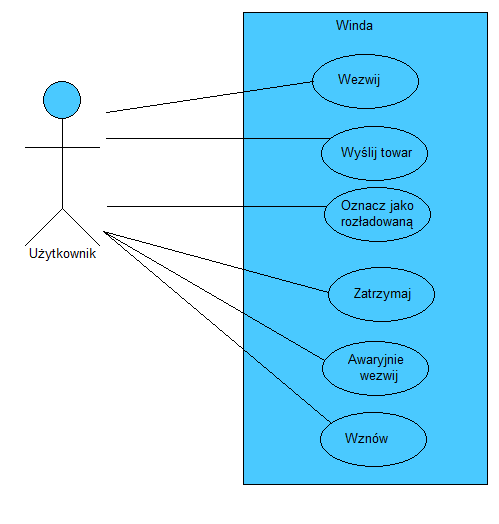
\includegraphics{images/useCase.png}    	
	\textbf{Scenariusze} \\
	\begin{itemize}
		\item Wezwij windę - scenariusz podstawowy
		\begin{itemize}
			\item warunek wstępny - winda jest na innym piętrze niż użytkownik oraz została oznaczona jako rozładowana,
			\item użytkownik wciska przycisk \textbf{bring here},
			\item winda podjeżdża na odpowiednie piętro.
		\end{itemize}
		\item Wezwij windę - scenariusz alternatywny
		\begin{itemize}
			\item warunek wstępny - winda jest na innym piętrze niż użytkownik ale nie została oznaczona jako rozładowana,
			\item użytkownik wciska przycisk \textbf{bring here},
			\item winda czeka aż zostanie oznaczona jako rozładowana,
			\item winda podjeżdża na odpowiednie piętro.
		\end{itemize}
		\item Wyślij windę - scenariusz podstawowy
		\begin{itemize}
			\item warunek wstępny - winda jest na tym samym piętrze co użytkownik,
			\item użytkownik dokonuje załadunku windy,
			\item użytkownik zamyka drzwiczki,
			\item użytkownik wciska przycisk z odpowiednim numerem piętra,
			\item winda odjeżdża na odpowiednie piętro.
		\end{itemize}
		\item Wyślij windę - scenariusz alternatywny			
		\begin{itemize}
			\item jeśli w trakcie załadunku przekroczona zostanie ładowność windy zapali się kontrolka ostrzegawcza
			\textbf {overload} oraz ostanie odegrany dzwięk ostrzegawczy.
			Winda nie zostanie wysłana.
			Należy usunąć z windy część ładunku i ponownie posłać windę.
			\item jeśli użytkownik nie zamknie drzwiczek zapali się kontrolka ostrzegawcza \textbf{doors open}
			oraz zostanie odegrany dzwięk ostrzegawczy, winda nie zostanie wysłana.
			Należy zamknąć drzwiczki i ponownie posłać windę.
		\end{itemize}
		\item Oznacz windę jako rozładowaną - scenariusz podstawowy
		\begin{itemize}
			\item warunek wstępny - winda jest na tym samym piętrze co użytkownik,
			\item użytkownik rozładowuje windę,
			\item użytkownik zamyka drzwiczki,
			\item użytkownik wciska przycisk \textbf{ready},
			\item winda zostaje oznaczona jako rozładowana.
		\end{itemize}
		\item Oznacz windę jako rozładowaną - scenariusz alternatywny \\
			Sytuacje berzegowe oraz ich obsługa takie same jak w poprzednim scenariuszu
		
		\item Zatrzymaj 
		\begin{itemize}
			\item warunek wstępny - brak,
			\item użtkownik wciska przycisk \textbf{stop},
			\item winda natychmiast się zatrzymuje.
		\end{itemize}
		
		\item Wezwij awaryjnie
		\begin{itemize}
			\item warunek wstępny - wida została zatrzymana, lub bezpośrednio uruchomiona po awarii,
			\item użytkonik wciska przycisk \textbf{Emergency Bring Here},
			\item winda podjeżdża nawet jeśli jest przeciążona lub niezamknięta.
		\end{itemize}
		
		\item Wznów
		\begin{itemize}
			\item warunek wstępny - wida została zatrzymana, lub bezpośrednio uruchomiona po awarii,
			\item użytkownik sprawdza stan windy,
			\item użytkownik wciska przycisk \textbf{Emergency ready},
			\item winda jest gotowa do użycia.
		\end{itemize}
		
	\end{itemize}
    
\section{Architektura}
	Winda została zaprojektowan jako maszyna stanowa. \\	
	Winda posiada kilka detectorów:
	\begin{itemize}
		\item detektor stanu drzwiczek (otwarte/zamknięte)
		\item detektor obciążenia windy
		\item detektor wysokości na której znajduje się winda
	\end{itemize}
	a także efektorów:
	\begin{itemize}
		\item silnik windy - przemieszczanie góra / dół
		\item dzwonek - do powiadamiania o alarmach (przeciążenie / otwarte drzwiczki)
		\item didy LED - informujące o alarmach (przeciążenie / otwarte drzwiczki)
	\end{itemize}
	Ponadto winda posiada dwa parametry
	\begin{itemize}
		\item tabela wysokości pięter
		\item maksymalne dopuszczalne obciążenie
	\end{itemize}
	Uproszczony diagram stanów \\
	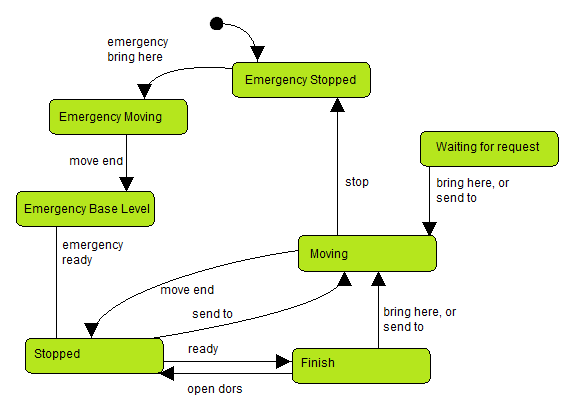
\includegraphics{images/simplifiedStateChart.png}
	
\section{Interfejs graficzny}
	
	
\section{Testy}
	Podczas testowania windy należy zwrócić uwagę na wszelkie sytuacje wyjątkowe.
	
	\subsection{Uruchomienie windy}
		\begin{enumerate}
			\item Próba wezwania windy na pierwszym piętrze
			\item Winda nie poinna się poruszyć
			\item Wciśnięcie przycisku \textbf{Emergency Ready}
			\item Próba wezwania windy na pierwszym piętrze 
			\item Winda powinna podjechać na pierwsze piętro
		\end{enumerate}
	\subsection{Załadunek windy}
		Warunek początkowy - winda jest poprawnie uruchomiona (przycisk Emergency Ready został już wciśnięty) - znajduje się na piętrze 0
		\begin{enumerate}
			\item Otwarcie drzwiczek,
			\item Próba wysłania windy na następne piętro,
			\item Winda nie powinna się poruszyć, powinna zapalić się lampka ostrzegawcza \textbf{doors open}, powinien zabrzmieć ostrzegawczy dzwonek.
			\item Zwiększenie obciążenia powyżej progu,
			\item Powinna zapalić się lapka \textbf{overload}, powinien zabrzmieć ostrzegawczy dzwonek
			\item Próba wysłania windy na następne piętro 
			\item Winda nie powinna się poruszyć, powinien zabrzmieć ostrzegawczy dzwonek
			\item Zdjęcie ciężaru poniżej limitu
			\item Lampka \textbf{overload} powinna zgasnąć
			\item Próba wysłania windy na następne piętro
			\item Winda nie powinna się poruszyć, powinien zabrzmieć ostrzegawczy dzwonek
			\item Zamknięcie drzwiczek
			\item Próba wysłania windy na następne piętro
			\item Winda powinna pojechać			
		\end{enumerate}
	\subsection{Wzywanie windy i oznaczanie jako rozładowanej} 
		Warunek początkowy - winda jest poprawnie uruchomiona, znajduje się na poziomie 0
		\begin{enumerate}
			\item wciśnięcie przycisku \textbf{bring here} na pierwszym piętrze
			\item winda powinna przyjechać na pierwsze piętro
			\item wciśnięcie przycisku \textbf{bring here} na poziomie 0
			\item winda nie powinna podjechać (powinna czekać na rozładowanie)
			\item wciścięcie przycisku \textbf{ready} na pierwszym piętrze
			\item wciścięcie przycisku \textbf{bring here} na poziomie 0
			\item winda powina zjechać na poziom 0
		\end{enumerate}
		
	\subsection{Przycisk stop i Emergency Ready}
		Warunek początkowy - winda jest poprawnie uruchomiona, znajduje się na poziomie 0
		\begin{enumerate}
			\item wciśnięcie przycisku stop
			\item próba wysłania windy na pierwsze piętro
			\item winda nie powinna się poruszyć, powinien zabrzmieć dzwonek ostrzegawczy
			\item próba przywołania windy na pierszym piętrze 
			\item winda nie powinna się poruszyć, powinien zbarzmieć dzwonek ostrzegawczy
			\item przyciśnięcie przycisku \textbf{Emergency Ready}
			\item próba wysłania windy na pierwsze piętro
			\item winda powinna się pojechać
			\item wciśnięcie przycisku stop, gdy winda znajduje się między piętrami.
			\item winda powinna się zatrzmać
			\item należy ponowić kroki 2-5
		\end{enumerate} 
		
	\subsection{Przycisk EmergencyBringHere}
		\begin{enumerate}
			\item pozostawnienie windy między piętrami (opisane w poprzednim teście)
			\item wciśnięcie przycisku \textbf{Emergency Bring Here}
			\item winda powinna zjechać na dolne piętro
			\item pozostawnienie windy na pierwszym piętrze z otwartymi drzwiczkami (zgodnie z powyższymi opisami)
			\item punkty 2,3
			\item pozostawnienie windy na pierwszym piętrze nie rozładowanej (zgodnie z powyższymi opisami)
			\item punkty 2, 3
			\item pozostawnienie windy przeciążonej na pierwszym piętrze (zgodnie z powyższymi opisami)
			\item punkty 2, 3
		\end{enumerate}


		
	
\section{Podsumowanie}
	Budowa oprogramowania przy pomocy środowiska IBM Raphsody 
	okazała się ciekawym i bardzo rozwijającym doświadczeniem.
	Dzięki możliwością wizunej budowy i analizy systemów opartych o maszyny stanowe pakiet ten idalnie 
	nadaje się do budowy systemów czasu rzeczywistego. Kolejnyą zaletą Raphsody jest zastosowanie 
	języków C++ oraz Java które są powszechnie znane i posiadają bardzo 
	duże wsparcie technicze i ogromne ilości bibliotek.
	Dzięki IBM Raphsody udało nam się stosunkow szybko stworzyć funkcjonalny i stabilny projekt.






\end{document}
